\documentclass[runningheads]{llncs}





\usepackage{color}

\usepackage{graphicx}
\usepackage{tikz}
\usepackage{calc}

\usepackage{amsmath, amssymb}
\DeclareMathOperator*{\argmin}{arg\,min}

\usepackage{wasysym}

\usetikzlibrary{automata}




\title{On the power of oritatami cotranscriptional folding with unary bead sequence\thanks{This work is supported in part by KAKENHI Grant-in-Aid for Challenging Research (Exploratory) No.~18K19779 and JST Program to Disseminate Tenure Tracking System No.~6F36 granted to S.~Z.~F. and S.~S.}
}
\author{
Szil\'{a}rd Zsolt Fazekas\inst{1} \and
Shinnosuke Seki\inst{2}\thanks{Corresponding author}}
\institute{
Akita University, 
Graduate School of Engineering Science, 
1-1 Tegate Gakuen-machi, Akita, 0108502, Japan \\
\email{szilard.fazekas@ie.akita-u.ac.jp}
\and
The University of Electro-Communications, 
Graduate School of Informatics and Engineering, 
1-5-1 Chofugaoka, Chofu, Tokyo, 1828585, Japan \\
\email{s.seki@uec.ac.jp}
}

\begin{document}

\maketitle

\begin{abstract}
We investigate simple oritatami systems in an attempt to establish lower bounds on the size and complexity of computationally universal systems. 
In particular, we look at oritatami systems, where the folding sequence consists of a number of beads of the same type and show that under reasonable assumptions, these systems are not universal.
\end{abstract}

%------------------------------------------------------
	\section{Introduction}
%------------------------------------------------------

Transcription is the first essential step of gene expression, when a DNA template sequence is copied into a complementary single stranded RNA sequence by a `copy machine' called RNA polymerase. 
The RNA strand is synthesized letter by letter according to the complimentarity relation ${\tt A} \rightarrow {\tt U}$, ${\tt G} \rightarrow {\tt C}$, ${\tt C} \rightarrow {\tt G}$, and ${\tt T} \rightarrow {\tt A}$ and folds up during a process called co-transcriptional folding.

In a recent breakthrough in molecular engineering by Geary, Rothemund and Andersen~\cite{RNAorigami} the co-transcriptional folding of RNA is controlled by careful design of the DNA template. As demonstrated in laboratory, this method, called RNA Origami, makes it possible to build rectangles out of RNA strands. 
Geary et al.~\cite{Oritatami} proposed a mathematical model for this process, called oritatami system.
It has been shown~\cite{Simulator} that the model is computationally universal by simulating cyclic tag systems introduced by Cook~\cite{Cook110}. 
The simulation involves a very large and complex oritatami system. 
One future direction of research is to find smaller universal oritatami system.

Closely related is the question of where not to look for universal systems, i.e., what are the limitations of simple oritatami system. 
In search for simple oritatami systems, there are a number of restrictions one can pose on them:
\begin{itemize}
\item bounds on the delay, the number of bead types or the arity;
\item bounds on the size of the primary structure or of the attraction rule set;
\item structural conditions on the primary structure or the attraction rule set.
\end{itemize}

%Rogers and Seki~\cite{SimpleSim} showed that certain OS with small delays are not universal.

%Han, Kim, Rogers and Seki\cite{SelfRemove} proved that it is possible to avoid self-attraction rules without changing the behavior of OS.

In this paper we start a new line of study which concerns the alphabet size for the primary structure, i.e., the number of bead types.

\begin{figure}[tb]
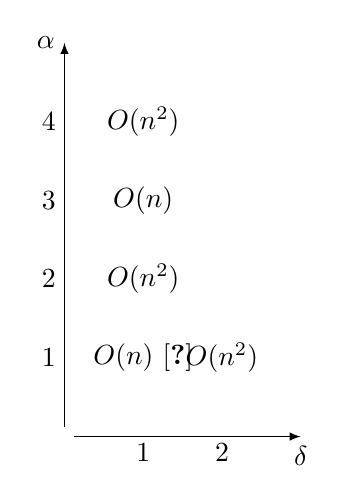
\begin{tikzpicture}

\node (origin) at (0, 0) {};

\draw[-latex] (origin) -- ++(0:3) node[below] {$\delta$}; 
\node at (1, -0.2) {1};
\node at (2, -0.2) {2};
\draw[-latex] (origin) -- ++(90:5) node[left] {$\alpha$}; 
\node at (-0.2, 1) {1};
\node at (-0.2, 2) {2};
\node at (-0.2, 3) {3};
\node at (-0.2, 4) {4};

%Results
\node at (1, 4) {$O(n^2)$};
\node at (1, 3) {$O(n)$};
\node at (1, 2) {$O(n^2)$};
\node at (1, 1) {$O(n)$ \cite{DemaineDNA24}};

\node at (2, 1) {$O(n^2)$};

\end{tikzpicture}
\caption{Summary of the results.}
\label{fig:summary}
\end{figure}

%------------------------------------------------------
	\section{Preliminaries}
%------------------------------------------------------
Let $\Sigma$ be a set of types of abstract molecules, or \textit{beads}. 
A bead of type $a \in \Sigma$ is called an $a$-bead. 
By $\Sigma^*$ and $\Sigma^\omega$, we denote the set of finite sequences of beads and that of one-way infinite sequences of beads, respectively. 
The empty sequence is denoted by $\lambda$. 
Let $w = b_1 b_2 \cdots b_n \in \Sigma^*$ be a sequence of length $n$ for some integer $n$ and bead types $b_1, \ldots, b_n \in \Sigma$. 
The \textit{length} of $w$ is denoted by $|w|$, that is, $|w| = n$. 
For two indices $i, j$ with $1 \le i \le j \le n$, we let $w[i..j]$ refer to the subsequence $b_i b_{i+1} \cdots b_{j-1}b_j$; if $i = j$, then $w[i..i]$ is simplified as $w[i]$. 
For $k \ge 1$, $w[1..k]$ is called a \textit{prefix} of $w$. 

Oritatami systems fold their transcript, which is a sequence of beads, over the triangular grid graph $\mathbb{T} = (V, E)$ cotranscriptionally. 
We designate one point in $V$ as the origin $O$ of $\mathbb{T}$. 
For a point $p \in V$, let $N_p^d$ denote the set of points which lie in the regular hexagon of radius $d$ centered at the point $p$. 
A directed path $P = p_1 p_2 \cdots p_n$ in $\mathbb{T}$ is a sequence of \textit{pairwise-distinct} points $p_1, p_2, \ldots, p_n \in V$ such that $\{p_i, p_{i+1}\} \in E$ for all $1 \le i < n$. 
Its $i$-th point is referred to as $P[i]$. 
Now we are ready to abstract RNA single-stranded structures in the name of conformation. 
A \textit{conformation} $C$ (over $\Sigma$) is a triple $(P, w, H)$ of a directed path $P$ in $\mathbb{T}$, $w \in \Sigma^*$ of the same length as $P$, and a set of h-interactions $H \subseteq \bigl\{\{i, j\} \bigm| 1 \le i, i+2 \le j, \{P[i], P[j]\} \in E \bigr\}$. 
This is to be interpreted as the sequence $w$ being folded along the path $P$ in such a manner that its $i$-th bead $w[i]$ is placed at the $i$-th point $P[i]$ and the $i$-th and $j$-th beads are bound (by a hydrogen-bond-based interaction) if and only if $\{i, j\} \in H$. 
The condition $i+2 \le j$ represents the topological restriction that two consecutive beads along the path cannot be bound. 
A \textit{rule set} $R \subseteq \Sigma \times \Sigma$ is a symmetric relation over $\Sigma$, that is, for all bead types $a, b \in \Sigma$, $(a, b) \in R$ implies $(b, a) \in R$. 
A bond $\{i, j\} \in H$ is \textit{valid with respect to $R$}, or simply $R$-valid, if $(w[i], w[j]) \in R$. 
This conformation $C$ is \textit{$R$-valid} if all of its bonds are $R$-valid. 
For an integer $\alpha \ge 1$, $C$ is \textit{of arity $\alpha$} if it contains a bead that forms $\alpha$ bonds but none of its bead forms more. 
By $\mathcal{C}_{\le \alpha}(\Sigma)$, we denote the set of all conformations over $\Sigma$ whose arity is at most $\alpha$; its argument $\Sigma$ is omitted whenever $\Sigma$ is clear from the context. 

The oritatami system grows conformations by an operation called elongation. 
Given a rule set $R$ and an $R$-valid conformation $C_1 = (P, w, H)$, we say that another conformation $C_2$ is an elongation of $C_1$ by a bead $b \in \Sigma$, written as $C_1 \xrightarrow{R}_b C_2$, if $C_2 = (P p, wb, H \cup H')$ for some point $p \in V$ not along the path $P$ and set $H' \subseteq \bigl\{ \{i, |w|+1\} \bigm| 1 \le i < |w|, \{P[i], p\} \in E, (w[i], b) \in R \bigr\}$ of bonds formed by the $b$-bead; this set $H'$ can be empty. 
Note that $C_2$ is also $R$-valid. 
This operation is recursively extended to the elongation by a finite sequence of beads as: for any conformation $C$, $C \xrightarrow{R}_\lambda^* C$; and for a finite sequence of beads $w \in \Sigma^*$ and a bead $b \in \Sigma$, a conformation $C_1$ is elongated to a conformation $C_2$ by $wb$, written as $C_1 \xrightarrow{R}_{wb}^* C_2$, if there is a conformation $C'$ that satisfies $C_1 \xrightarrow{R}_w^* C'$ and $C' \xrightarrow{R}_b C_2$. 

An \textit{oritatami system} (OS) $\Xi = (\Sigma, R, \delta, \alpha, \sigma, w)$ is composed of
\begin{itemize}
\item a set $\Sigma$ of bead types, 
\item a rule set $R \subseteq \Sigma \times \Sigma$, 
\item a positive integer $\delta$ called the \textit{delay}, 
\item a positive integer $\alpha$ called the \textit{arity}, 
\item an initial $R$-valid conformation $\sigma \in C_{\le \alpha}(\Sigma)$ called the \textit{seed}, upon which 
\item its (possibly infinite) \textit{transcript} $w \in \Sigma^* \cup \Sigma^\omega$ is to be folded by stabilizing beads of $w$ one at a time so as to minimize energy collaboratively with the succeeding $\delta{-}1$ nascent beads. 
\end{itemize}
The energy of a conformation $C = (P, w, H)$, denoted by $\Delta G(C)$, is defined to be ${-}|H|$; the more bonds a conformation has, the more stable it gets. 
The set $\mathcal{F}(\Xi)$ of conformations \textit{foldable} by the system $\Xi$ is recursively defined as: the seed $\sigma$ is in $\mathcal{F}(\Xi)$; and provided that an elongation $C_i$ of $\sigma$ by the prefix $w[1..i]$ be foldable (i.e., $C_0 = \sigma$), its further elongation $C_{i+1}$ by the next bead $w[i+1]$ is foldable if 
\begin{equation}\label{eq:OS_CF}
C_{i+1} \in \argmin_{
\substack{
C \in \mathcal{C}_{\le \alpha} s.t. \\
C_i \xrightarrow{R}_{w[i+1]}C \\
}
}
\min \Bigl\{ \Delta G(C') \Bigm|
C \xrightarrow{R}^*_{w[i+2...i+k]}C', k\le \delta, C' \in \mathcal{C}_{\le \alpha}
\Bigr\}.
\end{equation}
%
Then we say that the bead $w[i+1]$ and the bonds it forms are \textit{stabilized} according to $C_{i+1}$. 
Note that an arity-$\alpha$ oritatami system cannot fold any conformation of arity larger than $\alpha$. 
A conformation foldable by $\Xi$ is \textit{terminal} if none of its elongations is foldable by $\Xi$. 
The oritatami system $\Xi$ is \textit{deterministic} if for all $i \ge 0$, there exists at most one $C_{i+1}$ that satisfies \eqref{eq:OS_CF}. 
A deterministic oritatami system folds into a unique terminal conformation. 
An oritatami system with the empty rule set just folds into an arbitrary elongation of its seed nondeterministically. 
Thus, the rule set is always assumed to be non-empty. 

In the second half of this paper, we consider the unary oritatami system. 
An oritatami system is \textit{unary} if its bead type set $\Sigma$ is of size 1. 
Its sole bead type is denoted by $a$, that is, $\Sigma = \{a\}$. 
Its only possible rule is $(a, a)$ so that the non-empty rule set assumption implies that its rule set is $R = \{(a, a)\}$. 
Its transcript is a sequence of $a$-beads. 
That is to say, the behavior of a unary oritatami system is fully determined by the delay, arity, and seed. 





\begin{proposition}\label{prop:check_validity}
	For any rule set $R$, arity $\alpha$ and conformation $C = (P,w,H)$ it is possible to check whether $C$ is $R$-valid and whether $C\in \mathcal{C}_{\leq \alpha}$ in time $\mathcal{O}(|H|\cdot|w|\cdot|R|)$.
\end{proposition}
\begin{proof}
	To check whether $C$ is $R$-valid:
	\begin{enumerate}
		\item FOR each $(i,j)\in H$:
		\item \hspace{1cm} IF $(w[i],w[j])\notin R$ THEN answer NO and HALT
		\item answer YES and HALT
	\end{enumerate}	
	Checking the condition in 2. can be done in $\mathcal{O}(|w|\cdot|R|)$ time for any reasonable representation of $w$ and $R$, hence the whole process takes $\mathcal{O}(|H|\cdot |w|\cdot|R|)$ time.	
	To check the arity constraint $C\in \mathcal{C}_{\leq \alpha}$: 
	\begin{enumerate}
		\item FOR each $i\in \{1,\dots,|w|\}$:
		\item \hspace{1cm} IF $\mathrm{degree}(i)=|\{j | (i,j)\in H \}|>\alpha$ THEN answer NO and HALT
		\item answer YES and HALT
	\end{enumerate}	
	Checking the condition in 2. can be done in $\mathcal{O}(|H|)$ time for any reasonable representation of $H$, hence the whole process takes $\mathcal{O}(|w|\cdot|H|)$ time.
\end{proof}
\begin{theorem}\label{thm:OS_to_2dTM}
	There is an algorithm that simulates any oritatami system $\Xi = (\Sigma, R, \delta, \alpha, \sigma, w)$ in time $2^{\mathcal{O}(\delta)}\cdot |R|\cdot|w|$. 
\end{theorem}
\begin{proof}
	Take any step in the computation, up to which some $i \ge 0$ first beads of $w$ have been stabilized, with the last bead at a point $p$. 
	The number of all possible elongations of the current conformation by the next $\delta$-beads is $(6 \times 5^{\delta-1}) \times ((2^4)^{\delta-1} \times 2^5) \in 2^{O(\delta)}$. 
	By Proposition~\ref{prop:check_validity}, we can check for each of these elongations whether its arity is at most $\alpha$ or not and whether it is $R$-valid or not in time $\mathcal{O}((2^4)^{\delta-1}\cdot2^5\cdot \delta\cdot|R|)=2^{\mathcal{O}(\delta)}\cdot|R|$.  Therefore, the total running time is $2^{\mathcal{O}(\delta)}\cdot |R|\cdot|w|$.
\end{proof}

\begin{corollary}
	For fixed $\delta$ and $\alpha$, the class of problems solvable by oritatami systems $(\Sigma, R, \delta, \alpha, \sigma, w)$ is included in $\mathrm{DTIME}(n^3)$.
\end{corollary}
\begin{proof}
	The claim follows from Theorem~\ref{thm:OS_to_2dTM} and the fact that $|R|$ is implicitly bounded by $|w|^2$.
\end{proof}

%\begin{corollary}\label{polytranscript}
%	Let $k$ be a non-negative number. Let $\Sigma$, $H$, $\delta$, $\alpha$ be fixed and the transcript length bounded polynomially by the seed length, i.e., $|w|\in O(|\sigma|^k)$. Then, the language of seeds $\sigma$ accepted by an OS $(\Sigma, R, \delta, \alpha, \sigma, w)$ is in $\mathrm{DTIME}(|\sigma|^{2k})$.
%\end{corollary}

%If the transcript length is polynomially bounded by the seed length, than the accepted language is in $\mathrm{P}$. 

Because of the time hierarchy theorems, we know that $\mathrm{P}\subsetneq \mathrm{EXP}$, so we can conclude that OS which cannot deterministically fold transcripts of length exponential in the length of the seed are not computationally universal.

\section{Problem description}

In \cite{DemaineDNA24}, Demaine et al. proved that at delay 1 and arity 1, an oritatami system can fold upon the seed of size $n$ only the first $9n$ beads of a transcript deterministically. 
We consider this finiteness problem under various settings of the values of delay and arity. 
Results on this problem are summarized in Fig.~\ref{fig:summary}. 



\section{Case of $\delta = 1$}


\section{Case of $\delta \geq 2$}


\subsection{$\alpha = 1$, unary}

Let the point where the first transcript bead was fixed be $p$ and let $n=|\mathrm{seed}|+1$. We will argue about the situation when the first bead is stabilized outside $\hexagon_p^n$ (a hexagon of radius $n$). Let this be the $i$th bead of the transcript. Without loss of generality, we can translate the origin $(0,0)$ to the coordinates of bead $i-1$ (which is still in $\hexagon_p^n$), and we can assume that the bead outside the hexagon is fixed at $(1,1)$ (see Fig.~\ref{fig:hexagonOut}).
\begin{figure}
	\centering
	\includegraphics[width=0.3\linewidth]{./Fig/hexagonOut}
	\caption{$N_p^n$ and the position $(1,1)$ of the first bead fixed outside of it.}
	\label{fig:hexagonOut}
\end{figure}

In the elongation that places bead $i$ at $(1,1)$ there are two possibilities:
\begin{itemize}
	\item $i$ forms a bond with a bead at $(1,0)$.
	\item  $i$ does not bond to anything and $i+1$ is at $(2,1)$ bonding with a bead at $(2,0)$. If there is no bead at $(1,0)$, then placing $i$ at $(1,0)$ instead of $(1,1)$ results in the same number of bonds, leading to nondeterminism. Therefore, there has to be a bead at $(1,0)$ and it is inert, otherwise it would bond to $i$. This is analogous to case 1. below.%as in Fig.~\ref{fig:hexagonOut1}.
	\begin{figure}
		\centering
		\includegraphics[width=0.2\linewidth]{./Fig/hexagonOut1}
		%\caption{}
		\label{fig:hexagonOut1}
	\end{figure}
	
\end{itemize}
 
%The only position with which $(1,1)$ can form a bond is $(1,0)$. This means that there is a bead at $(1,0)$, which bonds to bead $i$, otherwise there are other conformations in which beads $i$ and $i+1$ add one bond to the conformation, making the behavior nondeterministic.

The next bead, $i+1$, can be fixed at $(2,1)$ or at $(0,1)$ as all other possibilities result in nondeterministic behavior immediately, so we have two cases.

\begin{enumerate}
	\item bead $i+1$ is fixed at $(2,1)$ and can bond with a bead at $(2,0)$. Now consider bead $i+2$. For $i+1$ to be fixed at $(2,1)$, $i+2$ needs to form a bond somewhere, otherwise $i+2$ could go to $(2,1)$ forming the bond with the bead at $(2,0)$ and there would be two conformations with the maximal $1$ bond. The only possibility is that there is a bead at $(3,0)$ and $i+2$ can bond with it when placed at $(3,1)$. We can apply the same argument inductively: there is some $m\geq 0$ such that grid points $(\ell,0)$ are occupied by active beads, for all $\ell\in \{2,\dots,2+m\}$, and there is no bead at $(3+m,0)$. Such an $m$ exists, and it is not greater than $n$. Then, bead $i+\ell$ is fixed at $(\ell+1,1)$ and bonds with $(\ell+1,0)$. However, bead $i+2+m$ cannot be fixed anywhere, because $i+2+m$ and $i+3+m$ can only add one bond to the conformation, and that is possible either with $i+2+m \rightarrow (2+m,1)$, $i+3+m \rightarrow (3+m,1)$ or with $i+2+m \rightarrow (2+m,2)$, $i+3+m \rightarrow (2+m,1)$. 
	\begin{figure}
		\centering
		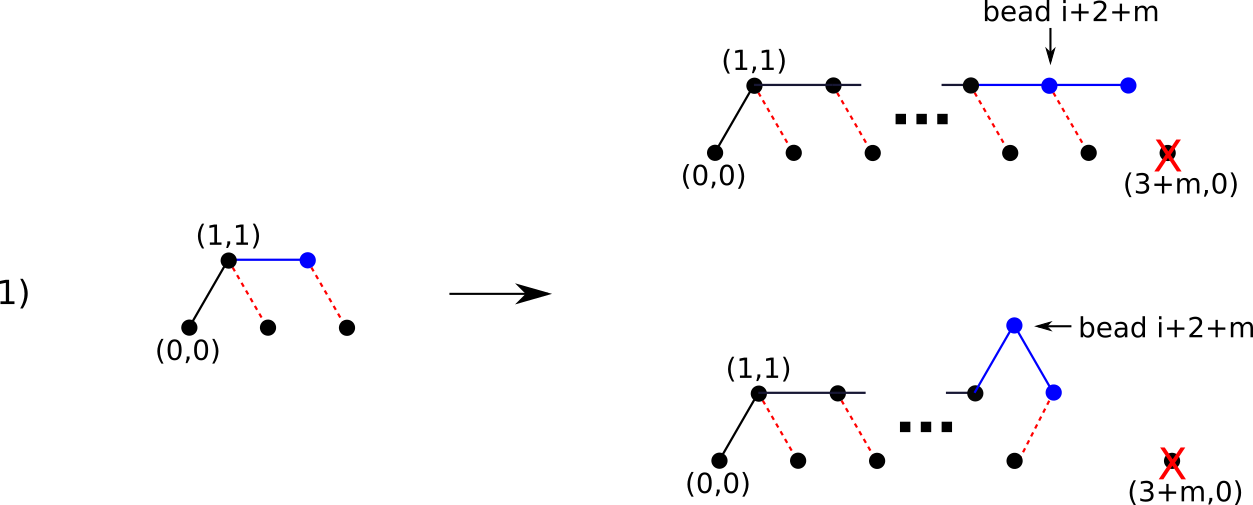
\includegraphics[width=0.6\linewidth]{./Fig/hexagonOut2}
		\caption{}
		\label{fig:hexagonout2}
	\end{figure}
	
	\item bead $i+1$ is fixed at $(0,1)$. This is only possible if
	\begin{enumerate}
		\item there is an inactive bead at $(-1,0)$ and an active one at $(-2,0)$. This case is symmetrical to (1).
		\item there is no bead at $(-1,0)$, bead $i+1$ can bond with bead $i-1$ at $(0,0)$ and the bead $i+2$ can be placed at $(-1,0)$ where it can bond with $(-2,0)$, $(-2,-1)$ or $(-1,-1)$. This leads to nondeterminism, because bead $i$ at $(-1,0)$ and bead $i+1$ at $(0,1)$ has two bonds, just as the original conformation.
		\item there is a bead at $(-1,0)$ and bead $i+1$ can bond with that or with bead $i-1$ at $(0,0)$. However, this means that placing bead $i$ at $(0,1)$ at bead $i+1$ at $(1,1)$ creates the same number of hydrogen bonds, thus resulting in bead $i$ not being placed deterministically.
		
	\end{enumerate}
\end{enumerate}




\begin{figure}
	\centering
	%\includegraphics[width=0.3\linewidth]{./hexagonOut1}
	%\hspace{10mm} %
	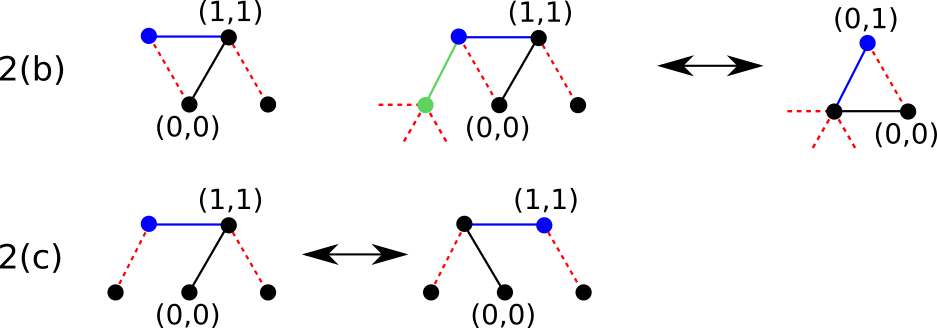
\includegraphics[width=0.6\linewidth]{./Fig/hexagonOut3}
	
	\caption{}
	\label{fig:hexagonOut2}
\end{figure}

  
\end{document}
